\documentclass[11pt,a4paper]{article}
\usepackage{times}

\usepackage{tikz}
\usetikzlibrary{positioning, fit,  shapes.geometric, arrows.meta}
\tikzset{
	node distance=1cm and 1.5cm,
	every text node part/.style= {
		align=center
	},
	word/.style= {
		blue,
		font=\itshape,
	},
	layer/.style= {
		rectangle, 
		black,
		draw
	},
	every node/.style ={anchor=base},
	every matrix/.style={ampersand replacement=\&, rounded corners=5pt, draw, column sep=15, row sep=15},
	refnode/.style={font={\footnotesize}, inner sep=0,outer sep=0, draw, red},
}

\newcommand{\refnode}[3][]{
\node(#3ref)[#1,refnode]{\ref{#2}};
\draw[red] (#3ref) to (#3);
}
\newcommand{\refnodeAR}[3][]{\refnode[above right=0.5 of #3]{#2}{#3}}
\newcommand{\refnodeBR}[3][]{\refnode[below right=0.5 of #3]{#2}{#3}}


\begin{document}
	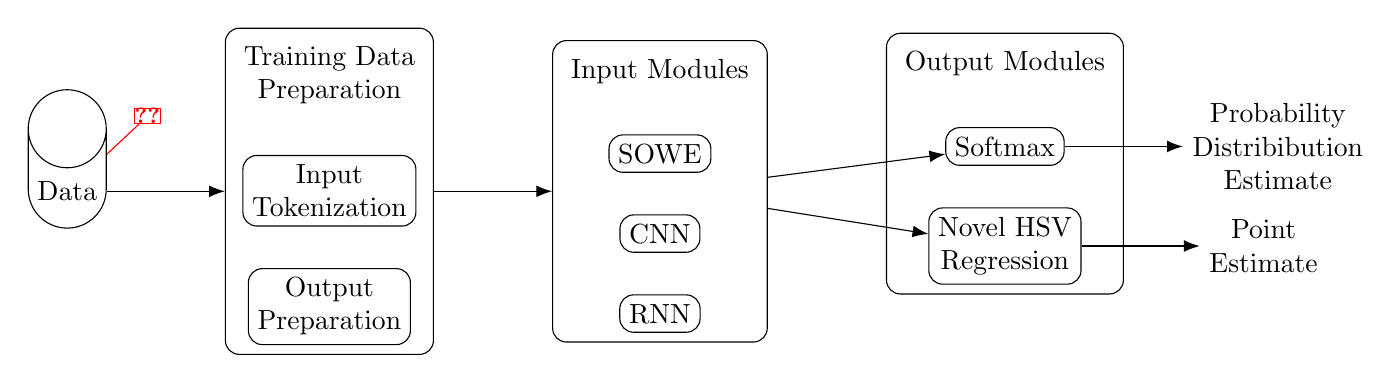
\begin{tikzpicture}
		\node (data) [cylinder, shape border rotate=90, draw, minimum height=5 em] {Data};
		
		\refnodeAR{foo}{data};

		\node (prep) [matrix, right = of data] {
				\node{Training Data \\ Preparation}; \\
				\node[draw]{Input\\Tokenization};\\
				\node[draw]{Output\\Preparation}; \\
			};
		
		\node (input) [matrix, right = of prep] {
			\node{Input Modules}; \\
			\node[draw]{SOWE};\\
			\node[draw]{CNN}; \\
			\node[draw]{RNN}; \\
		};
		
		\node (output) [matrix, right = of input, yshift=1em] {
			\node{Output Modules}; \\
			\node(softmax)[draw]{Softmax}; \\
			\node(hsvreg)[draw]{Novel HSV \\ Regression}; \\
		};
		\node(dist)[right=of softmax]{Probability\\Distribibution\\Estimate};
		\node(point)[right=of hsvreg]{Point\\Estimate};
		
		\draw[-{Latex[length=2mm]}] (data) to (prep);
		\draw[-{Latex[length=2mm]}] (prep) to (input);
		\draw[-{Latex[length=2mm]}] (input) to (softmax);
		\draw[-{Latex[length=2mm]}] (input) to (hsvreg);
		\draw[-{Latex[length=2mm]}] (softmax) to (dist);
		\draw[-{Latex[length=2mm]}] (hsvreg) to (point);
	\end{tikzpicture}
	
	
	\section{Zaa}\label{foo}
	sds
	\ref{foo}
\end{document}